\chapter{Bilancio delle Forze e dei Momenti}

%In questo capitolo estenderemo al caso tridimensionale i concetti e le idee già introdotte in 1D. Ovviamente ci troveremo di fronte ad una maggiore complessità analitica e ad un superiore ricchezza fisica da modellare.
Una volta fissata una configurazione $\Omega$ e una deformazione $\fb(\Omega)$,  affrontiamo il problema di modellare le interazioni meccaniche che le accompagnano, sia tra parti di $\Omega$ che tra $\Omega$ e l'ambiente circostante.  


\section{Sistemi di forze}
I tipi più semplici di interazioni meccaniche sono descritti dalle \textit{forze}. Nel tempo sono state sviluppate varie nozioni di  \textit{sistema di forze}, con l'obiettivo di  astrarre dall'esperienza, e quindi riflettere in un modello, un insieme di tratti salienti  delle azioni sul corpo e sull'ambiente in esame, sia separatamente, sia quando entrino in contatto. 

Il mondo intorno a noi offre esempi di azioni di \textit{superficie} su un corpo, come l'azione del vento su una vela; e azioni di \textit{volume} a distanza, come la gravità. La creazione di una nozione di sistema di forze che tenga conto in modo efficiente di tali interazioni superficie-contatto e volume-distanza, così come la creazione della relativa nozione di tensione, è essenzialmente dovuta ad \textsc{Leonhard Euler} (1707--1783, in italiano noto come Eulero) e \textsc{Augustin-Louis Cauchy} (1789--1857).


%\section{Sistemi di forze}
Data una configurazione $\Omega$, un sistema di forze (di Cauchy) si compone  formalmente di due campi:
\begin{itemize}
	\item le forze a \textit{distanza} $\bb(\xb)$  che agiscono in $\Omega$;
	\item le forze di \textit{contatto} $\sb(\xb)$, che agiscono sulla frontiera di $\Omega$.
\end{itemize}
Le forze a distanza hanno le dimensioni fisiche di una forza per unità di volume, ragion per cui sono talvolta chiamate forze di volume; le forze di contatto hanno  hanno le dimensioni fisiche di una forza per unità di superficie. 

Scelta una configurazione $\Omega$, definiamo \textit{risultante} delle forze che agiscono in $\bar{\Omega}$ come
\begin{definition}
	\begin{equation}
	\rb(\Omega)=\int_{\Omega}\bb(\xb) +\int_{\partial\Omega}\sb(\xb);
\end{equation}
\end{definition}
introduciamo inoltre il \textit{momento  risultante} rispetto al punto $\xb_0$ come
\begin{definition}
	\begin{equation}
\mb_{\xb_0}(\Omega)= \int_{\Omega}(\xb -\xb_0)\times \bb(\xb)+\int_{\partial\Pi}(\xb -\xb_0)\times \sb(\xb).
\end{equation}
\end{definition}


\section{Le azioni interne: la tensione}
%Come anticipato nel modello 1D, la caratterizzazione delle azioni interne qualifica il tipo di modello continuo che si introduce; noi limiteremo la nostra trattazione a quello di Cauchy. 
Cruciale nella descrizione dei corpi continui \textit{à la} Cauchy è la nozione di azione interna (o interazione di contatto). L'idea, che risale ad Eulero, è quella di considerare, all'interno dell'insieme $\Omega$, una sua parte e rendersi conto questa scambia con la parte complementare delle interazioni, che vanno caratterizzate. Questa caratterizzazione qualifica in maniera specifica la classe di corpi continui che consideriamo. In questa trattazione ci occuperemo solo dei cosiddetti \textit{continui di Cauchy}, che però non estinguono la classe di modelli esistenti per caratterizzare le interazioni di contatto.

Assegnata una configurazione $\Omega$, immaginiamo di separare in due parti la regione in questione tramite una superficie orientabile $\Sigma$, di normale $\nb$; denotiamo con $\Omega^-$ la parte che ha normale uscente $\nb$ in $\Omega \cap \Sigma$ e con $\Omega^+=\Omega\setminus\Omega^-$.  Fissiamo un punto $\xb$ in $\Omega \cap \Sigma$. La parte $\Omega^-$ scambia con $\Omega^+$, attraverso $\xb$, delle azioni interne, nella forma di interazioni di contatto, che occorre caratterizzare.

Per farlo, consideriamo per $\xb$ una palla $B(\xb, \varepsilon)$ di raggio $\varepsilon$ e valutiamo il risultante e il momento risultante delle forze che la regione $\Omega^+$ esercita su $\Omega^-$ attraverso la superficie $\Sigma \cap  B(\xb,\varepsilon)$:
\begin{equation}
\rb\big(\xb, \Sigma\cap B(\xb,\varepsilon)\big), \qquad \mb_\xb\big(\xb, \Sigma\cap B(\xb,\varepsilon)\big).
\end{equation}

\begin{figure}
	\centering
	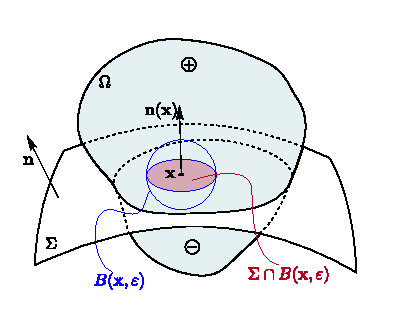
\includegraphics[scale=1.2]{figure/equilibrio/eulero3d}
	\caption{}
	\label{fig:eulero3d}
\end{figure}


Assumiamo, secondo il cosiddetto \textit{postulato di Cauchy}, che per ogni $\xb\in \Sigma$ esista $\tb(\xb; \Sigma)$ tale che
\begin{definition}
	\begin{equation}
\lim_{\varepsilon\to 0}\frac{\rb\big(\xb, \Sigma\cap B(\xb,\varepsilon)\big)}{A\big( \Sigma\cap B(\xb,\varepsilon)}=\tb(\xb, \Sigma)
\end{equation}
\end{definition}
e
\begin{definition}
	\begin{equation}
	\lim_{\varepsilon\to 0}\frac{\mb_\xb\big(\xb, \Sigma\cap B(\xb,\varepsilon)\big)}{A\big(\xb, \Sigma\cap B(\xb,\varepsilon)}=\mathbf{0},
\end{equation}
\end{definition}
dove $A\big(\Sigma\cap B(\xb,\varepsilon)$ è l'area della superficie $\Sigma\cap B(\xb,\varepsilon)$.

Il campo $\tb(\xb;\Sigma)$ è detto \textit{tensione} ed è dunque  la densità per unità di superficie del risultante delle azioni che la regione $\Omega^+$ esercita sulla regione $\Omega^-$ attraverso la
superficie $\Sigma$ in $\xb$. La densità del momento risultante è invece  assunta nulla. Questa scelta caratterizza di \textit{continui di Cauchy}. Esistono modelli in cui l'interazione di contatto non si riduce alla tensione, ma è più ricca, poiché si assume che sia non nulla anche la densità del momento risultate; ci si riferisce comunemente a questi modelli come \textit{continui  polari}.

È importante osservare che la tensione non dipende soltanto dal punto ma anche dalla superficie di taglio. Dimostreremo che:
\begin{itemize}
	\item $\tb$ dipende soltanto dalla normale $\nb$ a $\Sigma$ in $\xb$ e non da tutte le caratteristiche geometriche della superficie di taglio (\textit{Teorema di Hamel-Noll}\footnote{Questo teorema, nella maggior parte dei trattati, è considerato un postulato, spesso chiamato appunto \textit{postulato di Cauchy}. Da un punto di vista storico è corretto, perché Cauchy non lo dimostrò, ma lo assunse come dato. Tuttavia il risultato è un semplice risultato degli assiomi di Eulero, come mostrarono Hamel (parzialmente) e Noll.});
	\item $\tb$ dipende linearmente dalla normale $\nb$ (\textit{Teorema di Cauchy}).
\end{itemize}
Della seconda affermazione abbiamo dato una dimostrazione nel caso elementare 1D.

\subsection{L'assioma di Eulero}
%Per dimostrare i due punti occorrerà fare appello agli assiomi di Eulero, che bisogna precisare nel modello 3D. Preliminarmente 
Consideriamo una regione $\Pi \subset\Omega$, la cui frontiera $\partial\Pi$ sia composta da una parte esterna
\begin{equation}
\partial\Pi_e\coloneqq \partial\Pi\cap\partial \Omega
\end{equation}
 e una parte interna
\begin{equation}
\partial\Pi_i\coloneqq \partial\Pi\setminus\partial\Pi_e.
\end{equation}


\begin{center}
		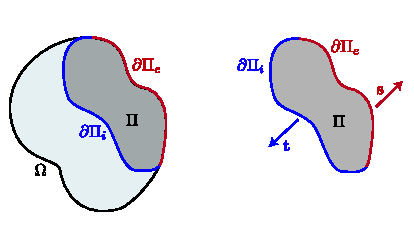
\includegraphics[scale=1.2]{figure/equilibrio/parti}
\end{center}


Per quanto detto, il risultante delle forze agenti su $\bar\Pi$ è
\begin{equation}
\rb(\Pi)=\int_{\Pi}\bb+ \int_{\partial \Pi_e} \sb +\int_{\partial\Pi_i} \tb(\cdot; \partial\Pi_i),
\end{equation}
mentre il momento risultante rispetto al polo $\xb_0$ è 
\begin{equation}
	\mb_{\xb_0}(\Pi)=\int_{\Pi}(\xb-\xb_0)\times\bb+ \int_{\partial \Pi_e} (\xb-\xb_0)\times\sb +\int_{\partial\Pi_i} (\xb-\xb_0)\times\tb(\cdot; \partial\Pi_i).
\end{equation}
Ammettiamo che sia valido il cosiddetto 
\begin{definition}
\textit{\textbf{Assioma di Eulero}}.	La configurazione  $\Omega$,  sotto l’azione delle forze di volume $\bb$, di superficie $\sb$ e delle tensioni $\tb$, è una configurazione di equilibrio se
	\begin{equation}\label{EulAx}
	\rb(\Pi)=\mathbf{0}, \qquad \mb_{\xb_0}(\Pi)=\mathbf{0}
\end{equation}
per ogni $\Pi\subset\Omega$ e per ogni $\xb_0$. 
\end{definition}

A partire dall'assioma di Eulero, che esprime una condizione di equilibrio globale, dedurremo delle condizioni di carattere puntuale. In particolare, utilizzeremo il seguente \textit{lemma di localizzazione}: se $B(\xb_0, \varepsilon)\coloneqq\{\xb \,:\, |\xb -\xb_0|\leq\varepsilon \}$ è la palla di raggio $\varepsilon$ centrata in $\xb$ e di volume $V\big(B(\xb_0, \varepsilon)\big)$, $\xb_0\in \Vc$ e $\gb$ una funzione continua in un intorno di $\xb_0$, allora
\begin{equation}\label{lemma3}
	\lim_{\varepsilon\to 0}\frac{1}{V\big(B(\xb_0, \varepsilon)\big)}\int_{B(\xb_0, \varepsilon)}\gb (\xb)=\gb(\xb_0).
\end{equation}

Utilizzeremo questo lemma per dimostrare il teorema di Hamel-Noll e il teorema di Cauchy.

\begin{remark}
Dimostriamo il lemma di localizzazione. 
Partiamo dall'espressione data:
\[
\frac{1}{V(B(\xb_0, \varepsilon))} \int_{B(\xb_0, \varepsilon)} \gb(\xb) \, \,\dd \xb.
\]
Poiché \( \gb \) è continua in \( \xb_0 \), possiamo esprimere \( \gb(\xb) \) come:
\[
\gb(\xb) = \gb(\xb_0) + (\gb(\xb) - \gb(\xb_0)).
\]
Sostituendo questa espressione nell'integrale, otteniamo:
\[
\begin{aligned}
\frac{1}{V(B(\xb_0, \varepsilon))} \int_{B(\xb_0, \varepsilon)} \gb(\xb) \, \,\dd \xb = &\frac{1}{V(B(\xb_0, \varepsilon))} \int_{B(\xb_0, \varepsilon)} \gb(\xb_0) \, \,\dd \xb \\
&+ \frac{1}{V(B(\xb_0, \varepsilon))} \int_{B(\xb_0, \varepsilon)} (\gb(\xb) - \gb(\xb_0)) \, \,\dd \xb.
\end{aligned}
\]
Il primo termine è semplice da calcolare:
\[
\frac{1}{V(B(\xb_0, \varepsilon))} \int_{B(\xb_0, \varepsilon)} \gb(\xb_0) \, \,\dd \xb = \frac{1}{V(B(\xb_0, \varepsilon))} \cdot V(B(\xb_0, \varepsilon)) \cdot \gb(\xb_0) = \gb(\xb_0).
\]
Ora consideriamo il secondo termine:
\[
\frac{1}{V(B(\xb_0, \varepsilon))} \int_{B(\xb_0, \varepsilon)} (\gb(\xb) - \gb(\xb_0)) \, \,\dd \xb.
\]
Poiché \( \gb \) è continua in \( \xb_0 \), per ogni \( \delta > 0 \), esiste un \( \varepsilon > 0 \) sufficientemente piccolo tale che:
\[
|\gb(\xb) - \gb(\xb_0)| < \delta \quad \text{per ogni} \quad \xb \in B(\xb_0, \varepsilon).
\]
Questo ci permette di stimare il secondo termine:
\[
\left| \frac{1}{V(B(\xb_0, \varepsilon))} \int_{B(\xb_0, \varepsilon)} (\gb(\xb) - \gb(\xb_0)) \, \,\dd \xb \right| \leq \frac{1}{V(B(\xb_0, \varepsilon))} \int_{B(\xb_0, \varepsilon)} |\gb(\xb) - \gb(\xb_0)| \, \,\dd \xb.
\]
Poiché \( |\gb(\xb) - \gb(\xb_0)| < \delta \) per ogni \( \xb \in B(\xb_0, \varepsilon) \), otteniamo:
\[
\frac{1}{V(B(\xb_0, \varepsilon))} \int_{B(\xb_0, \varepsilon)} |\gb(\xb) - \gb(\xb_0)| \, \,\dd \xb \leq \delta.
\]

Poiché \( \delta \) può essere reso arbitrariamente piccolo scegliendo \( \varepsilon \) sufficientemente piccolo, concludiamo che:
\[
\lim_{\varepsilon \to 0} \frac{1}{V(B(\xb_0, \varepsilon))} \int_{B(\xb_0, \varepsilon)} (\gb(\xb) - \gb(\xb_0)) \, \,\dd \xb = 0.
\]

Combinando i risultati otteniamo:
\[
\lim_{\varepsilon \to 0} \frac{1}{V(B(\xb_0, \varepsilon))} \int_{B(\xb_0, \varepsilon)} \gb(\xb) \, \,\dd \xb = \gb(\xb_0) + 0 = \gb(\xb_0).
\]

Pertanto, il teorema è dimostrato.


\end{remark}

\subsection{Il Teorema di Hamel-Noll}
Enunciamo il 
\begin{definition}
\textbf{\textit{Teorema di Hamel-Noll}} Date due superfici $\Sigma$ e $\hat\Sigma$ aventi almeno un punto in comune $\xb_0\in \Sigma\cap\hat{\Sigma}\subset\Omega$ e aventi la stessa normale $\nb$ in $\xb_0$, allora su una configurazione di equilibrio $\Omega$ per $\{\bb, \sb, \tb\}$,
\begin{equation}\label{HN0}
	\tb(\xb_0;\Sigma)=	\tb(\xb_0;\hat\Sigma).
\end{equation}
\end{definition}


In altri termini, la tensione dipende soltanto dalla normale; possiamo quindi definire
\begin{equation}
	\tb(\xb_0,\nb)\coloneqq \tb(\xb_0; \Sigma)=\tb(\xb_0; \hat\Sigma).
\end{equation}

Dimostriamo il teorema. La superficie $\Sigma$ divide in due parti, $\Omega^-$ e $\Omega^+$ la regione $\Omega$; analogamente, la superficie $\hat{\Sigma}$ divide la regione $\Omega$ in due parti, $\hat\Omega^-$ e $\hat\Omega^+$. Consideriamo il semi-cilindro $C_\varepsilon$ avente asse passante per $\xb_0$, base circolare di raggio $\varepsilon$ ortogonale a $\nb$ e distante $\varepsilon^2$ da $\nb$ e contenuta in $\Omega^-\cap \hat{\Omega}^-$

Definiamo
\begin{equation}
P_{\varepsilon}\coloneqq C_\varepsilon\cap \Omega^-, \qquad \hat{P}_{\varepsilon}\coloneqq C_\varepsilon\cap \hat\Omega^-
\end{equation}
le parti del semi-cilindro contenute in $\Omega^-$ e $\hat\Omega^-$. 


\begin{center}
	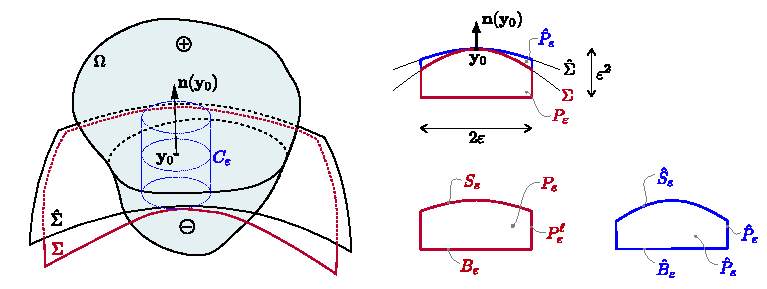
\includegraphics[scale=1.2]{figure/equilibrio/hamelnoll}
\end{center}

Scriviamo l'equilibrio a traslazione di $P_{\varepsilon}$:
\begin{equation}\label{rHN}
\rb(P_\varepsilon)=\int_{P_\varepsilon}\bb+\int_{B_\varepsilon}\tb(\cdot; B_\varepsilon)+\int_{P^\ell_\varepsilon}\tb(\cdot; P^\ell_\varepsilon)+\int_{S_\varepsilon}\tb(\cdot; \Sigma)=\mathbf{0},
\end{equation}
dove $B_\varepsilon$ è la base e $P^\ell_\varepsilon $ la superficie laterale di $P_\varepsilon$,  mentre $S_\varepsilon\coloneqq P_\varepsilon\cap\Sigma$ la ``base'' superiore, che si ottiene intersecando  $P_{\varepsilon}$ con la superficie $\Sigma$. Osserviamo che il volume $V(P_\varepsilon)$ è dell'ordine $O(\varepsilon^4)$, l'area $A(P_\varepsilon^\ell)$ dell'ordine $O(\varepsilon^3)$, l'area $A(B_\varepsilon)$ dell'ordine $O(\varepsilon^2)$ e l'area $A(S_\varepsilon)$ dell'ordine $\varepsilon^2$.

Dividiamo \eqref{rHN} per $A(S_\varepsilon)$ e riscriviamola in modo da poter applicare il lemma di localizzazione:
\begin{equation}
\begin{aligned}
&\frac{V(P_\varepsilon)}{A(S_\varepsilon)}\, \frac{1}{V(P_\varepsilon)}\int_{P_\varepsilon}\bb+
\frac{A(B_\varepsilon)}{A(S_\varepsilon)}\frac{1}{A(B_\varepsilon)}\int_{B_\varepsilon}\tb(\cdot ;B_\varepsilon)+\frac{A(P^\ell_\varepsilon)}{A(S_\varepsilon)}\int_{P^\ell_\varepsilon}\tb(\cdot ;P^\ell_\varepsilon)\\
&+\frac{1}{A(S_\varepsilon)}\int_{S_\varepsilon}\tb(\cdot; \Sigma)=\mathbf{0}.
\end{aligned}
\end{equation}
Nel far tendere $\varepsilon$ a zero, 
\begin{equation}
	\frac{V(P_\varepsilon)}{A(S_\varepsilon)}\to 0, \quad \frac{A(P^\ell_\varepsilon)}{A(S_\varepsilon)}\to 0, \quad \frac{A(B_\varepsilon)}{A(S_\varepsilon)}\to 1,\quad \frac{1}{A(S_\varepsilon)}\int_{S_\varepsilon}\tb(\cdot; S_\varepsilon)\to \tb(\xb_0; \Sigma)
\end{equation}
e dunque
\begin{equation}\label{HN1}
\tb(\xb_0; \Sigma)+\lim_{\varepsilon\to 0}\frac{1}{A(B_\varepsilon)}\int_{B_\varepsilon}\tb(\cdot ;B_\varepsilon)=\mathbf{0}.
\end{equation}

Richiedendo adesso che sia soddisfatta la condizione di equilibrio per $\hat P_\varepsilon$, si ha che 
\begin{equation}
\rb(\hat P_\varepsilon)=\int_{\hat P_\varepsilon}\bb+\int_{ B_\varepsilon}\tb(\cdot;  B_\varepsilon)+\int_{\hat P^\ell_\varepsilon}\tb(\cdot; \hat P^\ell_\varepsilon)+\int_{\hat S_\varepsilon}\tb(\cdot; \hat{\Sigma})=\mathbf{0}.
\end{equation}
Procedendo come per $P_\varepsilon$, si ottiene
\begin{equation}\label{HN2}
	\tb(\xb_0; \hat\Sigma)+\lim_{\varepsilon\to 0}\frac{1}{A(B_\varepsilon)}\int_{B_\varepsilon}\tb(\cdot ;B_\varepsilon)=\mathbf{0}.
\end{equation}
Dalle \eqref{HN1} e \eqref{HN2}  si ricava immediatamente la \eqref{HN0}.


\subsection{Il Teorema di Cauchy}
Enunciamo subito il teorema: 


\begin{definition}
	Sia $\Omega$ una configurazione di equilibrio per $\{\bb, \sb, \tb\}$. Allora la tensione dipende linearmente dalla normale; in particolare, esiste un campo tensoriale $\Tb \,:\, \Omega\to \Lin$, detto\textit{ tensore degli sforzi di Cauchy} tale che
\begin{equation}
\tb(\xb_0, \nb)= \Tb(\xb_0)\nb,
\end{equation}
per ogni $\xb_0\in\Omega$ e ogni vettore unitario $\nb$.
\end{definition}

Il teorema è una vera e propria pietra miliare nella meccanica dei continui, come lo stesso Cauchy riconobbe con orgoglio. La dimostrazione, pubblicata nel 1823, fa elegantemente uso di una costruzione basata su alcune proprietà geometriche del tetraedro, che richiameremo tra poco. Un innegabile valore di questa dimostrazione è di essere costruttiva, come vedremo: non soltanto produce un risultato di esistenza, a proposito del tensore degli sforzi, ma ne fornisce un'esplicita rappresentazione.

Nel seguito richiameremo prima alcune proprietà geometriche del tetraedro, indispensabili per la dimostrazione e poi stabiliremo un risultato preparatorio, che di solito va sotto il nome di \textit{Lemma di Cauchy}.

\subsubsection{Geometria del tetraedro} Consideriamo un tetraedro avente tre facce mutuamente ortogonali  di area $A_i$ e normale esterna $\eb_i$, mentre la faccia inclinata abbia area $A$ e normale esterna $\nb$, con $\nb\cdot\eb_i>0$ per $i=1,2,3$. Vogliamo dimostrare la seguente proprietà:
\begin{equation}\label{Ai}
	\frac{A_i}{A}=\nb\cdot \eb_i.
\end{equation}
Denominiamo con $\vb_i$ i tre vettori che vanno dall'origine all'intersezione $P_i$ del piano obliquo con gli assi paralleli a $\eb_i$. 

\begin{center}
	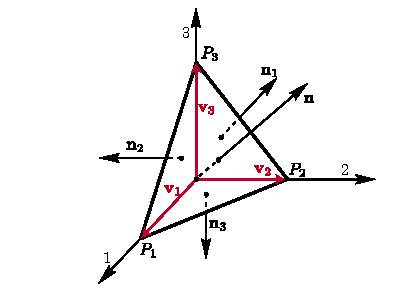
\includegraphics[scale=1.2]{figure/equilibrio/tetraedro}
\end{center}


Osserviamo che $\overrightarrow{P_1P_2}=\vb_2-\vb_1$ e $\overrightarrow{P_1P_3}=\vb_3-\vb_1$. Allora, per le proprietà del prodotto vettoriale, si ha che
\begin{equation}
	\begin{aligned}
	A \nb&=\frac12 \overrightarrow{P_1P_2}\times\overrightarrow{P_1P_3}=\frac12(\vb_1\times\vb_3-\vb_2\times\vb_1-\vb_1\times\vb_3)\\
	&=A_1 \eb_1+A_2 \eb_2+A_3 \eb_3,
	\end{aligned}
\end{equation}
da cui si deduce la \eqref{Ai}.

\subsubsection{Il Lemma di Cauchy}
Enunciamo il  lemma di Cauchy: 
\begin{definition}
La tensione $\tb(\xb_0,\nb)$ è una funzione dispari di $\nb$, ovvero
	\begin{equation}\label{lemmaC}
\tb\big(\xb_0,\nb(\xb_0)\big)=-\tb\big(\xb_0,-\nb(\xb_0)\big).
\end{equation} 
\end{definition}
L'interpretazione fisica è evidente: in un punto $\xb_0$, la tensione che si registra su un piano di normale $\nb$ è uguale e opposta a quella presente sul piano di normale $-\nb$. Non è altro che la formalizzazione del \textit{principio di azione e reazione}, nel presente contesto.

Per dimostrarlo usiamo un argomento simile a quello utilizzato per dimostrare il teorema di Hamel-Noll. Immaginiamo che la regione $\Omega$ sia separata in due da una superficie $\Sigma$ avente normale $\nb$ in $\xb_0$.  Consideriamo un semi-cilindro $C_\varepsilon$, avente raggio $\varepsilon$, base $B_\varepsilon$ situata a distanza $\varepsilon^2$ da $\xb_0$ e asse parallelo a $\nb$. Richiediamo che la parte $P_\varepsilon$ sia in equilibrio:
\begin{equation}
\rb(P_\varepsilon)=\int_{P_\varepsilon}\bb+\int_{B_\varepsilon}\tb(\cdot\,; - \nb)+\int_{P^\ell_\varepsilon}\tb(\cdot\,; \mb)+\int_{S_\varepsilon}\tb(\cdot\,; \nb)=\mathbf{0},
\end{equation}
dove $P^\ell_\varepsilon$ è la superficie laterale di $P_\varepsilon$, avente normale uscente $\mb$ e $S_\varepsilon=P_\varepsilon\cap \Sigma$. Dividendo per l'area $A(S_\varepsilon)$ e mandando $\varepsilon$ a zero, utilizzando il solito lemma di localizzazione, si trova
\begin{equation}
\tb(\xb_0, -\nb(\xb_0))+\tb(\xb_0, \nb(\xb_0))=\mathbf{0},
\end{equation}
donde il risultato atteso.

\subsubsection{L'argomento del tetraedro}
Veniamo dunque alla dimostrazione del teorema di Cauchy, tramite l'argomento del tetraedro.
Consideriamo una parte interna $\Tc_\varepsilon$ di $\Omega$, a forma di tetraedro avente tre spigoli passanti per $\xb_0$ e paralleli ad un sistema di assi cartesiani ortogonali prefissato arbitrariamente. Sia $\varepsilon$ la distanza tra $\xb_0$ e la faccia obliqua $S_\varepsilon$, di normale $\nb$, avente area $A(S_\varepsilon)$; le altre facce $S^i_\varepsilon$ abbiano area $A(S^i_\varepsilon)$ e normale uscente $-\eb_i$.

Imponiamo l'equilibrio del tetraedro:
\begin{equation}
\int_{\Tc_\varepsilon}\bb+ \int_{S_\varepsilon}\tb(\cdot, \nb)+\sum_{i=1}^{3}\int_{S_\varepsilon^i}\tb( \cdot, -\eb_i)=\mathbf{0}.
\end{equation}
Dividendo per $A(S_\varepsilon)$, abbiamo
\begin{equation}
\frac{V(\Tc_\varepsilon)}{A(S_\varepsilon)} \frac{1}{V(\Tc_\varepsilon)}	\int_{\Tc_\varepsilon}\bb+ \frac{1}{A(S_\varepsilon)} \int_{S_\varepsilon}\tb(\cdot, \nb)+\sum_{i=1}^{3}\frac{A(S^i_\varepsilon)}{A(S_\varepsilon)}\frac{1}{A(S^i_\varepsilon)}\int_{S_\varepsilon^i}\tb( \cdot, -\eb_i)=\mathbf{0}.
\end{equation}
Usando adesso il risultato \eqref{Ai} e mandando $\varepsilon$ a zero, poiché $V(\Tc_\varepsilon)=O(\varepsilon^3)$ e $A(S_\varepsilon)=O(\varepsilon^2)$, risulta che
\begin{equation}
\tb(\xb_0,\nb)=-\sum_{i=1}^{3}(\nb\cdot\eb_i)\tb(\xb_0, -\eb_i).
\end{equation}
Facendo adesso appello al lemma di Cauchy \eqref{lemmaC}, concludiamo che 
\begin{equation}
	\tb(\xb_0,\nb)=\sum_{i=1}^{3}(\nb\cdot\eb_i)\tb(\xb_0, \eb_i)=\left(\sum_{i=1}^{3}\tb(\xb_0, \eb_i)\otimes\eb_i\right) \nb.
\end{equation}
Ponendo
\begin{definition}
	\begin{equation}\label{Tb}
\Tb(\xb_0)\coloneqq \sum_{i=1}^{3}\tb(\xb_0, \eb_i)\otimes\eb_i,
\end{equation}
\end{definition}
possiamo allora scrivere
\begin{definition}
\begin{equation}\label{tTn}
\tb(\xb_0,\nb)= \Tb(\xb_0)\nb,
\end{equation}
\end{definition}
che ci mostra come il vettore tensione in $\xb_0$ relativo alla giacitura orientata da $\nb$ si ottiene dall'azione lineare su $\nb$ del valore in $\xb_0$ del campo tensoriale  $\Tb$, che rappresenta il cosiddetto \textit{tensore degli sforzi di Cauchy}. Come anticipato, la dimostrazione è costruttiva: di $\Tb$ si ottiene la rappresentazione esplicita \eqref{Tb}, che denuncia che per costruire il tensore degli sforzi in un punto è necessario conoscere il vettore della tensione su tre giaciture mutuamente ortogonali; nota questa, la tensione su qualunque piano è allora determinabile tramite la \eqref{tTn}.


\newpage
Scelta una base $\{\eb_i\}$, possiamo determinare le componenti di $\Tb$:
\begin{equation}
T_{ij}=\Tb\eb_j\cdot\eb_i=\tb(\cdot, \eb_i)\cdot\eb_i=t_i(\cdot, \eb_{j}).
\end{equation}
Dunque  $T_{ij}$ rappresenta  la $i$-esima componente della tensione su un piano di normale $\eb_j$.


\begin{center}
		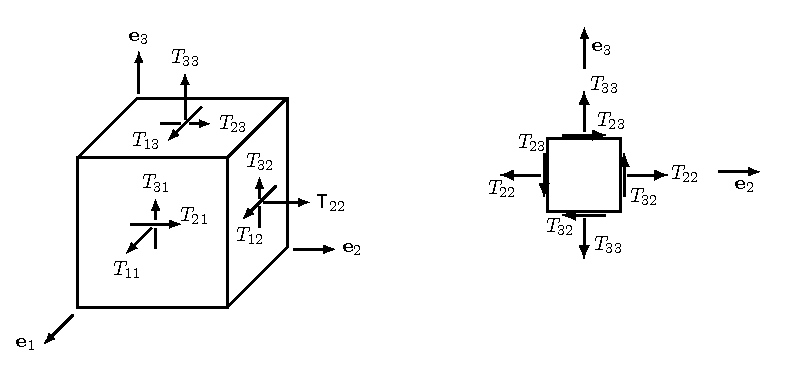
\includegraphics[scale=1]{figure/equilibrio/componenti_tensione}
\end{center}


\begin{exercise}
Nel punto $\xb_0$ è nota la tensione su tre piani di normale $\eb_i$ $(i=1,2,3)$:
\begin{equation}
	\begin{aligned}
		&\tb_1(\xb_0,\eb_1)=\alpha \eb_1-\beta \eb_3,\\
		&\tb_2(\xb_0,\eb_2)=\gamma \eb_2,\\
		&\tb_3(\xb_0,\eb_3)=-\alpha\eb_{1}+\beta\eb_2.
		\end{aligned}
\end{equation}
Determinare la tensione sul piano di normale $\nb=1/\sqrt{2}(\eb_1+\eb_2)$.
\begin{svolgimento}
Data la tensione su tre giaciture per $\xb_0$, la definizione di $\Tb$ ci consente di determinare il tensore di sforzo:
\begin{equation}
	\begin{aligned}&\Tb(\xb_0)=\sum_{i=1}^{3}\tb(\xb_0,\eb_{i})\otimes \eb_{i}=\\&=\tb_{1}(\xb_0,\eb_{1})\otimes \eb_{1}+\tb_{2}(\xb_0,\eb_{2})\otimes \eb_{2}+\tb_{3}(\xb_0,\eb_{3})\otimes \eb_{3}\\
	&=(\alpha \eb_{1}-\beta \eb_{3})\otimes \eb_{1}+\gamma \eb_{2}\otimes \eb_{2}+(-\alpha \eb_{1}+\beta \eb_{2})\otimes \eb_{3}.\end{aligned}
\end{equation}
La tensione sul piano di normale $\nb$ è allora
\begin{equation}
\tb(\xb_0,\nb)=\frac{1}{\sqrt{2}}\Tb(\xb_0)(\eb_1+\eb_2)=\frac{1}{\sqrt{2}}(\alpha \eb_1+\gamma \eb_2-\beta \eb_3).
\end{equation}
\end{svolgimento}
\end{exercise}



\section{Equazioni puntuali di equilibrio}
\subsection{Relazione di Cauchy per punti interni}
Consideriamo inizialmente un punto $\xb_0$ interno a $\Omega$, una configurazione di equilibrio per $\{\bb, \sb, \tb\}$. Sia $B(\xb_0,\varepsilon)$ la palla centrata in $\xb_0$, di raggio $\varepsilon$,  scelto piccolo abbastanza da garantire che $B(\xb_0,\varepsilon)\subset\Omega$. Per la palla in questione varrà l'assioma di Eulero
\begin{equation}
	\int_{B(\xb_0,\varepsilon)}\bb+\int_{\partial B(\xb_0,\varepsilon)}\tb (\cdot, \nb)=\mathbf{0},
\end{equation}
ovvero, facendo appello al teorema di Cauchy
\begin{equation}
		\int_{B(\xb_0,\varepsilon)}\bb+\int_{\partial B(\xb_0,\varepsilon)}\Tb\nb =\mathbf{0}.
\end{equation}
Facendo uso del teorema della divergenza, si ha che
\begin{equation}\label{eq1int}
	\int_{B(\xb_0,\varepsilon)}\bb+\Div\Tb=\mathbf{0}.
\end{equation}
Dividendo per $V(B(\xb_0,\varepsilon))$ e mandando a zero $\varepsilon$, facendo appello al lemma di localizzazione \eqref{lemma3}, si ottiene
\begin{definition}
	\begin{equation}\label{bDiv}
\bb(\xb_0)+\Div\Tb(\xb_0)=\mathbf{0},
\end{equation}
\end{definition}
per ogni punto $\xb_0$ interno a $\Omega$.

Scelta una base $\{\eb_i\}$, la \eqref{bDiv}, può essere scritta per componenti:
\begin{definition}
	\begin{equation}
	\begin{cases}b_{1}+\dfrac{\partial T_{11}}{\partial x_{1}}+\dfrac{\partial T_{12}}{\partial x_{2}}+\dfrac{\partial T_{13}}{\partial x_{3}}=0,\\[.3cm]
	b_{2}+	\dfrac{\partial T_{21}}{\partial x_{1}}+\dfrac{\partial T_{22}}{\partial x_{2}}+\dfrac{\partial T_{23}}{\partial x_{3}}=0,\\[.3cm]
	b_{3}+	\dfrac{\partial T_{31}}{\partial x_{1}}+\dfrac{\partial T_{32}}{\partial x_{2}}+\dfrac{\partial T_{33}}{\partial x_{3}}=0.
	\end{cases}
\end{equation}
\end{definition}


\subsection{Relazione di Cauchy per punti di frontiera}
Sia adesso $\xb_0$ un punto appartenente alla frontiera $\partial\Omega$. Consideriamo il semi-cilindro $C_\varepsilon$ con asse passante per $\xb_0$ e parallelo a $\nb(\xb_0)$, con base di raggio $\varepsilon$ che dista $\varepsilon^2$ da $\xb_0$. Sia $P_\varepsilon=\Omega\cap C_\varepsilon$. L'equilibrio a traslazione di $P_\varepsilon$ richiede che
\begin{equation}
\int_{P_\varepsilon}\bb+\int_{S_\varepsilon}\sb +\int_{B_\varepsilon}\Tb(-\nb)+\int_{P_\varepsilon^\ell}\Tb \mb,
\end{equation} 
dove $B_\varepsilon$ è la base di $P_\varepsilon$, $P_\varepsilon^\ell$ la superficie laterale di normale uscente $\mb$ e $S_\varepsilon=\partial P_\varepsilon\cap\partial\Omega$. Dividendo per $A(B_\varepsilon)$ e mandando $\varepsilon$ a zero si ottiene, col solito argomento,
\begin{equation}
\sb(\xb_0)-\Tb(\xb_0)\nb(\xb_0)=\mathbf{0},
\end{equation}
ovvero
\begin{definition}
	\begin{equation}\label{Tns}
\Tb(\xb_0)\nb(\xb_0)=\sb(\xb_0)
\end{equation}
\end{definition}
per ogni $\xb_0\in\partial\Omega$. Il campo di sforzo $\Tb(\xb_0)$ è da intendersi come l'estensione al bordo di $\Tb$, in realtà definito  sull'aperto $\Omega$. La \eqref{Tns} stabilisce che, sulla frontiera di $\Omega$, il vettore tensione è pari alla forza di contatto esercitata dall’ambiente esterno sul corpo.

\subsection{La simmetria del tensore degli sforzi}
Non abbiamo fin qui fatto alcun uso della seconda delle condizioni \eqref{EulAx}, che valgono quando un sistema di forze è bilanciato.  Riprendiamola applicandola ad una palla $B(\xb_0,\varepsilon)$ di raggio $\varepsilon$ centrata in $\xb_0$ e facendo uso del teorema di Cauchy:
\begin{equation}
	\int_{ B(\xb_0,\varepsilon)}\xb \times \bb +	\int_{ \partial B(\xb_0,\varepsilon)}\xb \times \sb=	\int_{ B(\xb_0,\varepsilon)}\xb \times \bb +	\int_{ \partial B(\xb_0,\varepsilon)}\xb \times \Tb \nb=\mathbf{0}.
\end{equation}
Sia $\wb\in \Vc$ un vettore \textit{costante} e $\Wb\in \Skw$ tali che $\wb\times\ab=\Wb\ab$ per ogni $\ab\in\Vc$; banalmente si ha che
\begin{equation}
\int_{ B(\xb_0,\varepsilon)}\wb\cdot \xb \times \bb +	\int_{ \partial B(\xb_0,\varepsilon)}\wb\cdot \xb \times \Tb \nb=0.
\end{equation}
Poiché $\wb\cdot \xb\times \bb=\bb\cdot \wb\times\xb =\bb\cdot \Wb \xb$ e $\wb\cdot \xb \times \Tb \nb=\Tb\nb\cdot \Wb \xb$, possiamo scrivere
\begin{equation}
\int_{ B(\xb_0,\varepsilon)}\bb\cdot \Wb \xb+	\int_{ \partial B(\xb_0,\varepsilon)}\nb\cdot\Tb^\top \Wb \xb=\int_{ B(\xb_0,\varepsilon)}\Div(\Tb^\top \Wb \xb)=0,
\end{equation}
dove, per l'ultima eguaglianza, abbiamo adoperato il teorema della divergenza. Usando l'identità
\begin{equation}
\Div (\Ab \gb)=(\Div \Ab^\top)\cdot \gb+\Ab^\top\cdot \nabla \gb,
\end{equation}
valida per qualunque $\Ab \in \Lin$ e $\gb \in \Vc$, possiamo scrivere 
\begin{equation}
\Div(\Tb^\top \Wb \xb)=(\Div \Tb)\cdot \Wb \xb+\Tb\cdot\Wb
\end{equation}
e dunque 
\begin{equation}
\int_{ B(\xb_0,\varepsilon)}(\bb+\Div\Tb)\cdot \Wb \xb +\Tb\cdot\Wb=0.
\end{equation}
Osserviamo che, in virtù della \eqref{eq1int}, il primo addendo è nullo. Dividendo per il volume della palla e mandando $\varepsilon$ a zero, si ottiene allora
\begin{equation}
	\Tb(\xb_0)\cdot \Wb=0.
\end{equation}
Vista l'arbitrarietà di $\Wb\in\Skw$, se ne conclude che 
\begin{definition}
	\begin{equation}
	\Tb(\xb_0)\in \Sym.
\end{equation}
\end{definition}
Dunque un campo di sforzo associato a un sistema di forze bilanciato deve avere valori \textit{simmetrici}.

\vspace{.2cm}
In conclusione, il tensore degli sforzi di Cauchy associato ad una configurazione di equilibrio per una terna $\{\bb, \sb, \tb\}$ deve soddisfare le seguenti condizioni:
\begin{definition}
	\begin{equation}\label{pstat}
	\begin{cases}
		\begin{array}{ll}
			\Div\Tb +\bb= \mathbf{0}, & \qquad \text{in}\;\; \Omega \\
			\Tb=\Tb^\top,  & \qquad \text{in}\;\; \Omega \\
			\Tb\nb=\sb, & \qquad \text{su}\;\; \partial\Omega,
		\end{array}
	\end{cases}
\end{equation}
\end{definition}

Dati una configurazione $\Omega$ e un sistema di forze esterne $\{\bb, \sb\}$ si dice che un campo di sforzo $\Tb$ su $\Omega$ risolve il relativo \textit{problema statico} se le \eqref{pstat}  sono soddisfatte. Le \eqref{pstat}  costituiscono un sistema di 3 equazioni differenziali alle derivate parziali, nelle 6 incognite date dalle componenti di sforzo; in generale, questo problema non ammette soluzione unica.




\begin{exercise}
	Il tensore degli sforzi nel cubo $\Omega=(-1,1)\times(-1,1)\times(-1,1)$ ha una matrice rappresentativa
	\begin{equation}
		[\Tb]=\left[\begin{array}{ccc}
			\sigma x_2 x_3	& \sigma x_2^2 & \sigma(x_1-x_3)  \\
			\sigma x_2^2	& \sigma x_2 & 0 \\
			\sigma(x_1-x_3)  	&  0 &  \sigma x_3
		\end{array}\right].
	\end{equation}
	Sapendo che il cubo è in equilibrio, determinare le forze di volume e di superficie applicate.
	\begin{svolgimento}
		Viste le \eqref{bDiv}, si trova immediatamente
		\begin{equation}
			\begin{aligned}
				&	-b_1=(\Div \Tb)_1=T_{1j,j}=T_{11,1}+T_{12,2}+T_{13,3}=\sigma(2x_2-1),\\
				&-b_2=(\Div \Tb)_2=T_{2j,j}=T_{21,1}+T_{22,2}+T_{23,3}=\sigma,\\
				&-b_3=(\Div \Tb)_3=T_{3j,j}=T_{31,1}+T_{32,2}+T_{33,3}=2\sigma
			\end{aligned}
		\end{equation}
		ovvero
		\begin{equation}
			\bb = \sigma\Big(  (1-2x_2)\eb_1+\eb_2+2\eb_3 \Big).
		\end{equation}
		Per determinare le forze di superficie applicate sulla faccia di normale $\eb$, occorre valutare $\Tb$ sul piano $x_1=1$ e poi vederne l'azione su $\nb =\eb_1$:
		\begin{equation}
			[\Tb(1,x_2,x_3)]=\left[\begin{array}{ccc}
				\sigma x_2 x_3	& \sigma x_2^2 & \sigma(1-x_3)  \\
				\sigma x_2^2	& \sigma x_2 & 0 \\
				\sigma(1-x_3)  	&  0 &  \sigma x_3
			\end{array}\right]
			\left[\begin{array}{c}
				1\\
				0\\
				0
			\end{array}\right]	=\sigma
			\left[\begin{array}{c}
				x_2x_3\\
				x_2^2\\
				1-x_3
			\end{array}\right],
		\end{equation}
		e così via per le altre facce.
	\end{svolgimento}
\end{exercise}



\begin{exercise}
	Fissato un sistema di coordinate cartesiane $(x_1, x_2, x_3)$, si consideri il sistema di coordinate cilindriche $(\rho, \theta, z)$, $x_1=\rho\cos\theta$, $x_2=\rho\sin\theta$, $x_3=z$ e l'associata base ortonormale $\{\eb_\rho, \eb_\theta, \eb_z\}$,
	\begin{equation}
		\eb_\rho=\cos\theta\eb_1+\sin\theta\eb_2, \quad \eb_\theta=-\sin\theta\eb_1+\cos\theta\eb_2, \quad \eb_z=\eb_3.
	\end{equation}
	Il cilindro cavo
	\begin{equation}
		(R-\delta)<\rho< R, \quad 0\leq\theta<2\pi, \quad -L/2< z< L/2
	\end{equation}
\begin{center}
	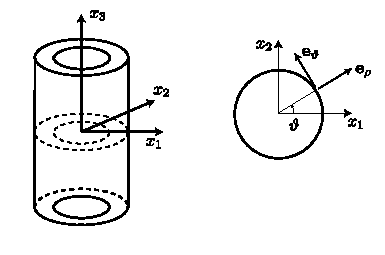
\includegraphics[scale=1.2]{figure/equilibrio/esempio13d}
\end{center}
	sia soggetto allo sforzo 
\begin{equation}
	\Tb=2\sigma \eb_\vartheta\otimes \eb_\vartheta+\sigma \eb_z \otimes \eb_z +\frac{\tau}{R}\rho (\eb_\vartheta\otimes\eb_z+\eb_z\otimes\eb_\vartheta).
\end{equation}
%	$\Tb$ rappresentato nella base $\{\eb_\rho, \eb_\theta, \eb_z\}$ dalla matrice
%	\begin{equation}
%		[\Tb]=\sigma\left[
%		\begin{array}{ccc}
%			0 & 0& 0\\
%			0 & 2 & 0\\
%			0& 0& 1
%		\end{array}
%		\right]+
%		\frac{\tau}{R}\left[
%		\begin{array}{ccc}
%			0 & 0& 0\\
%			0 & 0 & \rho\\
%			0& \rho& 0
%		\end{array}
%		\right].
%%	\end{equation}
	\begin{enumerate}
		\item Scrivere le componenti cartesiane del campo vettoriale della tensione $\tb$ sulla sezione trasversale di normale esterna $\eb_3$ per l'origine.
		% $t_x= -\tau y/R, t_y=\tau x/R, t_z=\sigma$
		\item Sulla sezione longitudinale del cilindro di normale esterna $\eb_1$ per l'origine, calcolare le componenti cartesiane del vettore  risultante $\rb$ delle tensioni e del vettore momento risultante $\mb_0$ rispetto all'origine.
		%\begin{equation}
		%m_x= -\frac{2}{3}\tau\delta R L \left( \left( \frac{\delta}{R}\right)^2 -3\frac{\delta}{R}+1 \right), \quad m_y=m_z=0.
		%\end{equation}
	\end{enumerate}
\begin{svolgimento}
\begin{enumerate}
	\item La tensione sulla faccia di normale $\eb_3$ si trova grazie al teorema di Cauchy
	\begin{equation}
	\Tb \eb_z=\sigma \eb_z +\frac{\tau}{R}\rho \eb_\vartheta=\frac{\tau}{R}(-x_2\eb_1+x_1\eb_2)+\sigma \eb_3.
	\end{equation}
\item 
Occore determinare la tensione sulle superfici $\Sc_1$ e $\Sc_2$, di normale $\eb_1$.
\begin{center}
	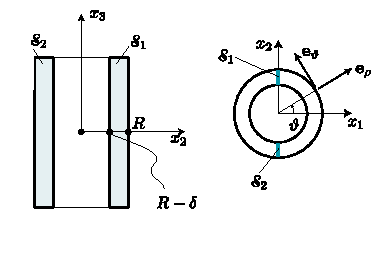
\includegraphics[scale=1.2]{figure/equilibrio/esempio13d_1}
\end{center}
Risulta che
\begin{equation}
\Tb \eb_1=2\sigma \sin^2\vartheta \eb_1-2\sigma\sin\vartheta\cos\vartheta\eb_2-\frac{\tau}{R}\rho \sin\vartheta\eb_3.
\end{equation}
Su $\Sc_1$ abbiamo che $\vartheta=\pi/2$ e dunque
\begin{equation}
\tb_1=\Tb \eb_1|_{\vartheta=\pi/2}=2\sigma\eb_1-\frac{\tau}{R}\rho \eb_3,
\end{equation}
mentre su $\Sc_2$ abbiamo che $\vartheta=-\pi/2$ e dunque
\begin{equation}
	\tb_2=\Tb \eb_1|_{\vartheta=-\pi/2}=2\sigma\eb_1+\frac{\tau}{R}\rho \eb_3.
\end{equation}
Il risultante è allora
\begin{equation}
	\rb=\int_{-L/2}^{L/2}\int_{R-\delta}^{R}\tb_{1}+\tb_{2}=4\sigma \delta L \eb_1.
\end{equation}
Per calcolare il momento risultante rispetto all'origine, occorre determinare il braccio: essendo la posizione del generico punto
\begin{equation}
	\xb=\rho\cos\vartheta\eb_1+\rho \sin\vartheta\eb_2+x_3\eb_{3},
\end{equation}
su $\Sc_1$ abbiamo
\begin{equation}
	\xb_1 = \rho\, \eb_2+x_3\,\eb_3,
\end{equation}
mentre su $\Sc_1$ abbiamo
\begin{equation}
	\xb_2= -\rho\, \eb_2+x_3\,\eb_3.
\end{equation}
Il momento risultante è allora
\begin{equation}
\mb_0=\int_{-L/2}^{L/2}\int_{R-\delta}^R\xb_1\times \tb_1+\xb_2\times \tb_2=-\frac23 \frac{\tau}{R}(R^3-(R-\delta)^3)\,\eb_1.
\end{equation}
\end{enumerate}

\end{svolgimento}
\end{exercise}

\begin{exercise}
	%Villaggio
	Sia $\bar\Tb$ lo sforzo medio in una configurazione $\Omega$ soggetta a forze di volume $\bb$ e di contatto $\sb$ in equilibrio. Usando il teorema della divergenza, dimostrare che
	\begin{equation}
		\bar\Tb=\frac{1}{\textrm{vol}(\Omega)}\left( \int_{\Omega}\xb\otimes\bb+\int_{\partial\Omega}\xb\otimes\sb \right),
	\end{equation}
	dove $\xb$ è il generico punto di $\Omega$.
\begin{svolgimento}
Innanzitutto osserviamo che
\begin{equation}
\int_{\partial\Omega}\xb\otimes \sb=\int_{\partial\Omega}\xb\otimes \Tb \nb,
\end{equation}
su cui cerchiamo di applicare il teorema della divergenza. Lavoriamo per componenti. Dati un vettore $\ab\in \Vc$ e in tensore $\Ab \in \Lin$,
\begin{equation}
(\ab \otimes \Ab \nb)_{ij}=a_i A_{jk}n_k
\end{equation}
e dunque, per il teorema della divergenza
\begin{equation}
	\int_{\partial\Omega}a_i A_{jk}n_k=\int_{\Omega}(a_i A_{jk}),_{k}.
\end{equation}
Abbiamo che 
\begin{equation}
(a_i A_{jk}),_{k}=a_{i,k}A_{jk}+a_i A_{jk,k}=\big((\nabla \ab)\, \Ab^\top\big)_{ij}+(\ab \otimes \Div \Ab)_{ij}
\end{equation}
e dunque
\begin{equation}
\int_{\partial\Omega}\ab \otimes \Ab \nb =\int_{\Omega}(\nabla \ab)\, \Ab^\top+\ab \otimes \Div \Ab.
\end{equation}
Utilizziamo questo risultato generale con $\ab=\xb$ e $\Ab =\Tb$:
\begin{equation}
	\int_{\partial\Omega}\xb \otimes \Tb \nb =\int_{\Omega}(\nabla \xb)\, \Tb^\top+\xb \otimes \Div \Ab=\int_{\Omega}\Tb -\xb \otimes \bb,
\end{equation}
da cui 
\begin{equation}
\int_{\Omega}\xb \otimes \bb +\int_{\partial \Omega}\xb \otimes\sb=\int_{\Omega}\Tb,
\end{equation}
e dunque segue immediatamente il risultato ricercato.
\end{svolgimento}
\end{exercise}

\section{Tensioni principali}
Il vettore della tensione che si registra su un piano di normale $\nb$ ha, in generale, due componenti: una diretta come $\nb$ 
\begin{equation}
\sigmab\coloneqq\sigma\nb \quad\sigma\coloneqq \tb(\nb) \cdot \nb
\end{equation}
detta \textit{tensione normale} ed una perpendicolare ad $\nb$
\begin{equation}
\taub\coloneqq \tb(\nb) -\sigmab.
\end{equation}
detta \textit{tensione tangenziale}. Ci si può chiedere se esistano giaciture per cui la tensione sia puramente normale. Per rispondere alla domanda occorre risolvere il problema
\begin{equation}\label{autov}
	\tb(\nb)=\sigmab \quad  \Longleftrightarrow\quad \Tb \nb =\sigma \nb.
\end{equation} 
La \eqref{autov}$_2$ mostra che per rispondere alla nostra domanda occorre risolvere un \textit{problema agli autovalori}. Dato che $\Tb$ è un tensore simmetrico, ci si può appellare al teorema spettrale per concludere che i suoi autovalori sono tutti reali e gli autovettori mutuamente ortogonali. Dunque esistono tre giaciture, ortogonali tra di loro, sulle quali la tensione è solamente normale. Del tensore di sforzo si può allora dare la \textit{rappresentazione spettrale} seguente:
\begin{definition}
	\begin{equation}
	\mathbf{T}=\sum_{i=1}^3\lambda_i\mathbf{n}_i\otimes\mathbf{n}_i
\end{equation}
\end{definition}
dove $\lambda_i$ sono gli autovalori (reali) di $\Tb$ e $\nb_i$ i corrispondenti autovettori (ortonormali). Gli autovalori sono chiamanti \textit{tensioni principali} e gli autovettori \textit{direzioni principali}. Conveniamo di numerare le tensioni principali come segue:
\begin{equation}
	\lambda_1\leq\lambda_2\leq\lambda_3.
\end{equation}
Allora $\lambda_3$ è la massima tensione normale e $\lambda_1$ la minima.

L'inviluppo delle direzioni principali individua tre famiglie di curve mutuamente ortogonali, note come \textit{linee isostatiche}. Su queste curve, le tensioni sono esclusivamente normali, pertanto il materiale viene semplicemente compresso o teso lungo tali direzioni. Inoltre, queste linee rappresentano i punti di massima trazione e compressione.

La natura ottimizza l'utilizzo della materia costruendo strutture che possiedono la forma, le dimensioni e la resistenza necessarie con la minima quantità di massa possibile. Un esempio evidente di questo principio si osserva nelle \textit{ossa lunghe}, come il femore o l'omero, dove le trabecole ossee si dispongono lungo le linee isostatiche.

La disposizione delle trabecole ossee lungo le linee isostatiche era stata osservata molto prima che Cauchy descrivesse formalmente lo stato di sforzo. Tuttavia, in tempi più recenti, si è visto  che molti organismi viventi sono in grado di modellarsi e rimodellarsi continuamente in risposta a segnali derivanti dallo stato di sforzo locale. Questi segnali sono generati dai carichi esterni che l'organismo deve sostenere. Prendendo ancora come esempio le ossa lunghe, questo processo di adattamento è reso possibile dall'azione combinata degli \textit{osteoclasti}, che demoliscono il tessuto osseo, e degli \textit{osteoblasti}, che lo ricostruiscono.


\begin{figure}
	\centering
	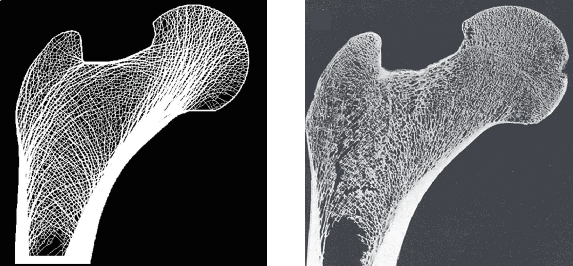
\includegraphics[width=0.8\linewidth]{figure/cinematica/osso_direzprinc}
	\caption{Struttura trabecolare in un femore prossimale, determinata tramite un modello (sinistra) e reale (destra). La disposizione delle trabecole ossee segue le linee isostatiche. (Tratto da M. Huo, S. He, Y. Zhang, Y. Feng, J. Lu, Simulation on bone remodeling with stochastic nature of adult and elderly using topology optimization algorithm, Journal of Biomechanics, Volume 136, 2022.)}
	\label{fig:ossodirezprinc}
\end{figure}



%La meccanica dei tessuti biologici rappresenta uno dei numerosi ambiti della scienza in cui una comprensione approfondita dello stato di sforzo è fondamentale.  Questo è particolarmente importante per comprendere come le strutture biologiche, come le ossa, rispondano e si adattino ai vari carichi che sopportano durante la loro vita. La capacità di adattamento e ottimizzazione osservata nei tessuti biologici  offre anche preziose intuizioni che possono essere applicate  nella progettazione di materiali artificiali bio-inspirati.

%
%\section{Stati di sforzo elementari}
%
%\subsubsection{Pressione idrostatica}
%
%\subsubsection{Trazione/compressione semplice}
%
%\subsubsection{Taglio semplice}
%
%
%
%\section{Lavoro di un sistema di forze}\label{Lav3D}
%Nella meccanica ci sono due modi diversi per fornire una rappresentazione matematica del concetto di forza: il primo consiste nel rappresentarla tramite un \textit{vettore} applicato, un ente matematico avente  un'origine, un modulo, una direzione e un verso. L'estensione naturale ai mezzi continui porta alla definizione di campi vettoriali associati a misure, da cui le `forze di volume', `di superficie', `per unità di massa', etc.
%
%Il secondo modo, che risale almeno a \textsc{Jean-Baptiste Le Rond d'Alembert} (1717--1783), è quello cui normalmente ci si riferisce come metodo dei lavori virtuali. Questo secondo modo è in realtà più naturale del primo, essendo una traduzione in termini matematici di ciò che comunemente si fa nell'esperienza per valutare una forza. Ad esempio, se si desidera conoscere la forza peso di un oggetto, l'operazione più naturale che si fa è `soppesarlo', ovvero imprimere uno spostamento (o una velocità) e valutare quanta `fatica' si fa nell'operazione: il nostro cervello non è in grado di valutare una forza, ma solo il lavoro che essa compie. Da un punto di vista matematico questa procedura si può descrivere così: ad un certo istante, si considera sul sistema $\Pc$ un campo vettoriale $\ub$ che definisce, a quell'istante, uno \textit{spostamento virtuale}; le forze che producono questo spostamento sono note se è noto il loro `lavoro virtuale'. 
%%Ancora più precisamente  --- e astrattamente  ---  si considera un insieme $\Uc$ di spostamenti virtuali $\delta\ub$, dove $\Uc$ è uno spazio dotato di norma, e si afferma di conoscere le forze esercitate su un sistema se esiste un funzionale lineare $\Lc(\Pc)[\delta\ub]$, il cui valore, per ogni $\delta\ub$, è uguale al lavoro virtuale prodotto dalle forze durante il moto definito da $\delta\ub$.
%
%%L'idea fondamentale che sta alla base di questo secondo modo di vedere le cose è quella di \textit{dualità}. Uno dei vantaggi di questo secondo modo di procedere risiede senz'altro nella possibilità di definire in maniera piuttosto libera lo spazio $\Uc$, in modo da avere una descrizione più o meno fine del moto del sistema: è quel che abbiamo fatto all'inizio dello studio della cinematica della trave, in cui lo spazio degli spostamenti virtuali è quello indotto dalla cinematica dei corpi a forma di trave, che richiedeva una descrizione dello spostamento dei punti della linea d'asse e della rotazione locale della sezione trasversale. Una volta fissato $\Uc$, l'insieme delle forze definisce a sua volta lo spazio vettoriale $\Uc^\star$, il \textit{duale} di $\Uc$.
%
%%Occorre ammettere che la nozione di funzionale lineare definito su uno spazio vettoriale è  più astratta e complessa di quella di un campo vettoriale, motivo per cui la prima descrizione della nozione di forza è quella che, almeno all'inizio, è prevalsa. Inoltre, nel momento in cui è apparsa questa idea, la nozione di dualità, che può essere vista come un precursore della nozione di \textit{misura} e di \textit{distribuzione}, non era ancora stata sviluppata appieno. Oggigiorno l'analisi funzionale e le sue applicazioni alla meccanica hanno fornito strumenti matematici notevoli alla nozione di dualità sicché, a partire almeno dalla metà del secolo scorso, l'utilizzo degli strumenti connessi all'idea di lavoro virtuale e dualità è stata estremamente feconda nello sviluppo delle teorie di campo.
%
%%In questo capitolo intendiamo mettere in luce gli aspetti meccanici che la nozione di dualità indotta da quella del lavoro virtuale  porta con sé, nel caso dei corpi continui a forma di trave.
%
%Di seguito utilizzeremo il concetto di \textit{lavoro virtuale}, che nel contesto della meccanica puntiforme può essere definito come segue: se $\pb$ è una forza che agisce su un punto e $\ub$ è un qualunque spostamento del punto (non necessariamente quello prodotto dalla forza $\pb$), allora la quantità $\pb \cdot \ub$ rappresenta il lavoro virtuale che la forza $\pb$ compie sullo spostamento $\ub$. In sostanza, il termine virtuale indica che non esiste necessariamente una ``corrispondenza'' tra forza e spostamento.
%
%
%\section{Equazione dei lavori virtuali}\label{ELV3Ds}
%Sia  $\Omega\supset\Pi$ soggetto ad un sistema di forze $(\bb, \sb)$; su $\Pi$ assumiamo che sia definito un campo di spostamento $\ub$. Si definisce lavoro esterno, compiuto dal sistema di forze sullo spostamento dato, 
%\begin{definition}
%	\begin{equation}
%	\Lc_e(\Omega)\coloneqq\int_{\Omega}\bb\cdot \ub+\int_{\partial \Omega}\sb\cdot \ub.
%\end{equation}
%\end{definition}
%che generalizza  il lavoro di un punto materiale.
%
%Diciamo che $\{\Eb, \ub\}$  è compatibile, o \textit{congruente}, se
%\begin{equation}
%	\Eb =\sym \nabla \ub,
%\end{equation}
%Consideriamo adesso la terna $\{\Tb, \bb, \sb\}$ di sforzo, forze di volume e di contatto; diciamo che la terna  è equilibrata se
%\begin{equation}
%	\begin{cases}
%		\begin{array}{ll}
%			\Div\Tb +\bb= \mathbf{0}, & \qquad \text{in}\;\; \Omega \\
%			\Tb = \Tb^\top, & \qquad \text{in}\;\; \Omega \\
%			\Tb\nb=\sb, & \qquad \text{su}\;\; \partial\Omega.
%		\end{array}
%	\end{cases}
%\end{equation}
%
%
%Vale il seguente 
%\begin{definition}
%	\textbf{\textit{Teorema dei Lavori Virtuali}}. Sia $\{\Eb, \ub\}$  una coppia congruente e sia $\{\Tb, \bb, \sb\}$ una terna equilibrata. Allora il \textit{lavoro virtuale esterno}
%	\begin{equation}\label{ELV3D}
%		\begin{aligned}
%			\Lc_e(\Omega)&\coloneqq\int_{\Omega}\bb\cdot \ub+\int_{\partial \Omega}\sb\cdot \ub
%		\end{aligned}
%	\end{equation}
%	è uguale al lavoro \textit{virtuale interno }
%	\begin{equation}
%		\Lc_i(\Omega)=\int_{\Omega}\Tb\cdot \Eb.
%	\end{equation}
%\end{definition}
%
%La dimostrazione è  solo una generalizzazione al caso 3D di quanto già visto nel contesto semplificato 1D, per la quale  è necessario usare la seguente identità:
%\begin{equation}
%	\int_\Omega\mathbf{T}\cdot\mathbf{E}=-\int_\Omega\mathrm{~div}\,\mathbf{T}\cdot\mathbf{u}+\int_{\partial\Omega}\mathbf{T}\mathbf{n}\cdot\mathbf{u}.
%\end{equation}
%Ovviamente, come nel caso 1D, valgono le seguenti proposizioni:
%\begin{definition}
%	\begin{equation}
%		\mathcal{L}_i=\mathcal{L}_e\quad\forall\{\mathbf{E},\mathbf{u}\}\text{ congruente}\quad\Longrightarrow\quad\{\mathbf{T},\mathbf{b},\mathbf{s}\}\text{ equilibrata}
%	\end{equation}
%\end{definition}
%e
%\begin{definition}
%	\begin{equation}
%		\mathcal{L}_i=\mathcal{L}_e\quad\forall\{\mathbf{T},\mathbf{b},\mathbf{s}\}\text{ equilibrata}\quad\Longrightarrow\quad\{\mathbf{E},\mathbf{u}\}\text{ congruente.}
%	\end{equation}
%\end{definition}
%Le dimostrazioni sono banali estensioni di quanto già discusso nella Sez. \ref{ELV1D}.
%


